\documentclass[12pt,a4paper]{book}
\raggedbottom

\usepackage{ugmath_notas}
\usepackage{float}
\usepackage{placeins}
\usepackage[labelfont=bf,labelsep=space]{caption}
\usepackage{pdfpages}
\usepackage{tikz-cd}
\usepackage{amsthm}
\renewcommand{\Tr}{\operatorname{Tr}}
\newcommand{\llaves}[1]{\{#1\}}
\newcommand{\parentesis}[1]{\left(#1\right)}
\newcommand{\corchetes}[1]{\left[#1\right]}
\newcommand{\llavesgrande}[1]{\big\{#1\big\}}
\newcommand{\llavesgrandes}[1]{\left\{#1\right\}}


\begin{document}
        
    
    \thispagestyle{empty}
    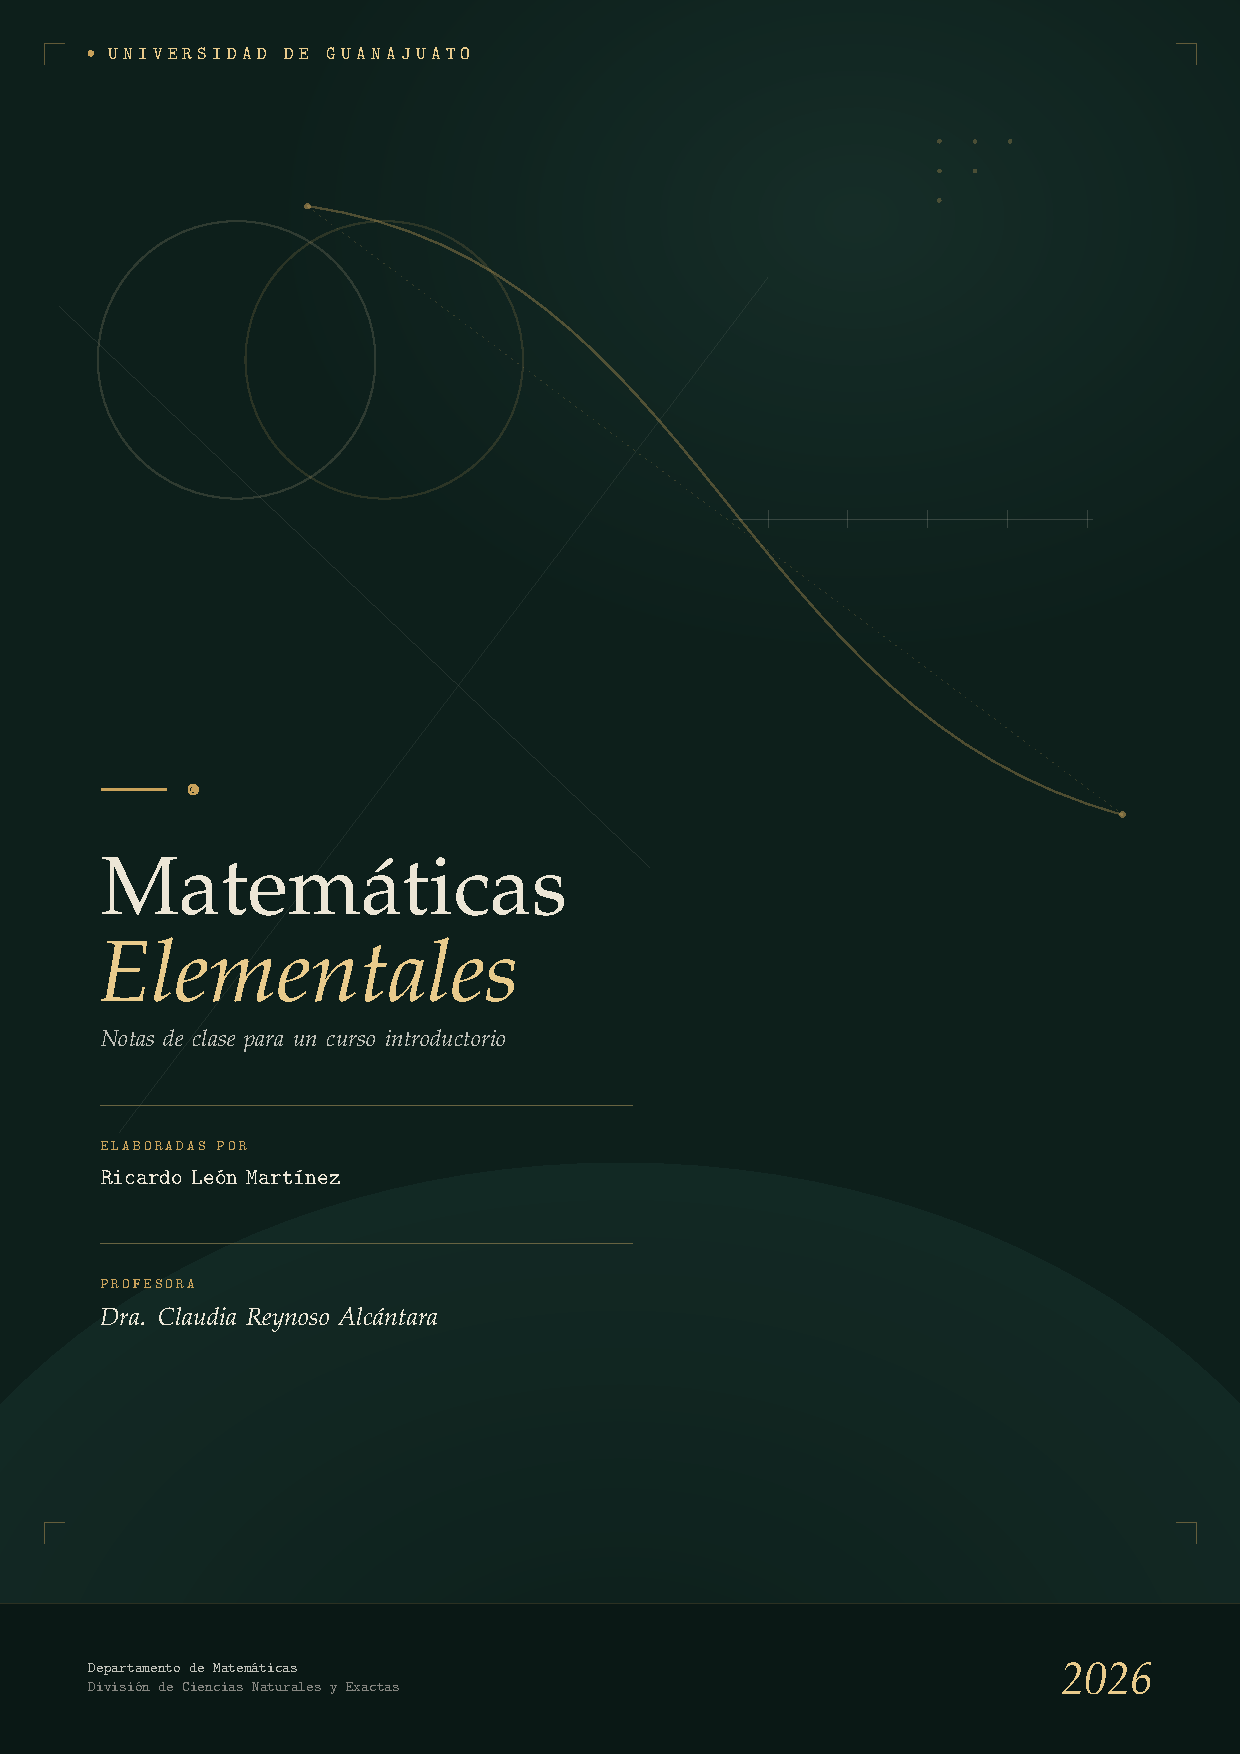
\includepdf[pages=1]{portada-matematicas-elementales.pdf}

    \begin{flushright}
      \thispagestyle{empty}

        \textit{Dedicado a todos aquellos que no creyeron\\
        que estas notas fueran a salir. (Uicab)}\\[1cm]

        \textbf{Ricardo}\\[0.3cm]
        \textit{A los tacos el paisa 2\\
        porque son unos rifados.\\
        A Román porque sufrió redactando\\
        estas notas.\\
        A Uicab por su libreta\\
        de lineal.\\
        Al grupo de todos ínfimos porque\\
        hacen más llevadera la universidad.\\
        Y a Sam, porque aunque no entienda\\
        del todo estas notas,\\
        siempre estuvo ahí.\\
        Y a Kaori, porque entre tareas, estrés\\
        y examenes, también estuvo ahí.}\\[1.2cm]
    \end{flushright}

    % ---------------- NOTA DE ERRORES ----------------

    \cleardoublepage
    \thispagestyle{empty}

    \begin{mdframed}[style=mdgreenbox]
        \begin{center}
        \small
        Estas notas fueron elaboradas con fines académicos.\\
        A pesar del cuidado puesto en su redacción,\\
        es posible que existan errores u omisiones.\\[0.3cm]

        Cualquier corrección, sugerencia o comentario será bienvenido
        en el correo: \\[0.3cm]

        ricardo.leon@cimat.mx
        \end{center}
    \end{mdframed}

    % -------------------------------------------------
    
    \setcounter{page}{1}
    \tableofcontents

\end{document}